\chapter{अंतरापृष्ठ, पृष्ठसक्रियक और कोलॉइड}\label{ch:b3:colloids}

मेयोनेज़ थोड़े-से जल और सिरके में कुछ माइक्रोमीटर चौड़े बूँदकों के रूप में परिक्षिप्त तेल है,
जिन्हें अंडे की ज़र्दी के लेसिथिन और प्रोटीन अलग-अलग रखते हैं। आरंभ में बहुत तेज़ी से
फेंटने पर, या तेल बहुत जल्दी डालने पर, यह एक तैलीय परत और एक जलीय परत में
फट जाता है: बूँदक आपस में मिल जाते हैं, और वह ऊर्जा, जो उन्हें अलग रखती थी, समाप्त हो जाती है।
दूध, कोहरा, स्याही, पेंट, रक्त और नदी का मटमैला जल
इसी प्रकार के पदार्थ हैं: अणुओं से कहीं बड़े और आँख से दिखने वाली किसी भी चीज़ से
कहीं छोटे कण या बूँदक, इतने अधिक कि उनके अधिकांश अणु
किसी अंतरापृष्ठ के निकट होते हैं। यह अध्याय अंतरापृष्ठों की ऊर्जा, उसे घटाने वाले
अणुओं, अंतरापृष्ठों द्वारा संभव होने वाले \omterm{def:b3:colloids:colloid}{कोलॉइडों}, और इस बात का विवेचन करता है कि
\omterm{def:b3:colloids:colloid}{कोलॉइडों} को क्या परिक्षिप्त रखता है या उन्हें स्कंदित करता है।

\begin{recall}
प्रथम वर्ष के खंड ने जलरागी शीर्ष और जलविरागी पुच्छ वाले अणु को उभयरागी
कहा, और लंदन अन्योन्यक्रियाओं तथा विलायकों के आपेक्षिक
परावैद्युतांक का वर्णन किया; विद्यालय के खंड के कक्षा 11 वाले भाग में साबुन में \omterm{def:b3:colloids:micelle}{मिसेल}
आए थे। द्वितीय वर्ष के खंड ने रासायनिक विभव, आयनिक सामर्थ्य और
सक्रियता को परिभाषित किया। \Cref{ch:b3:surfaces-catalysis} ने ठोसों पर \omterm{def:b3:surfaces-catalysis:adsorption}{अधिशोषण} का,
\cref{ch:b3:electrode-kinetics} ने \omterm{def:b3:electrode-kinetics:double-layer}{वैद्युत द्विपरत} और उसकी \omterm{def:b3:electrode-kinetics:double-layer}{डिबाई
लंबाई} का विवेचन किया। भौतिकी से: ब्राउनी गति, और किसी वक्र पृष्ठ के भीतर
का दाब।
\end{recall}

\begin{omfigure}
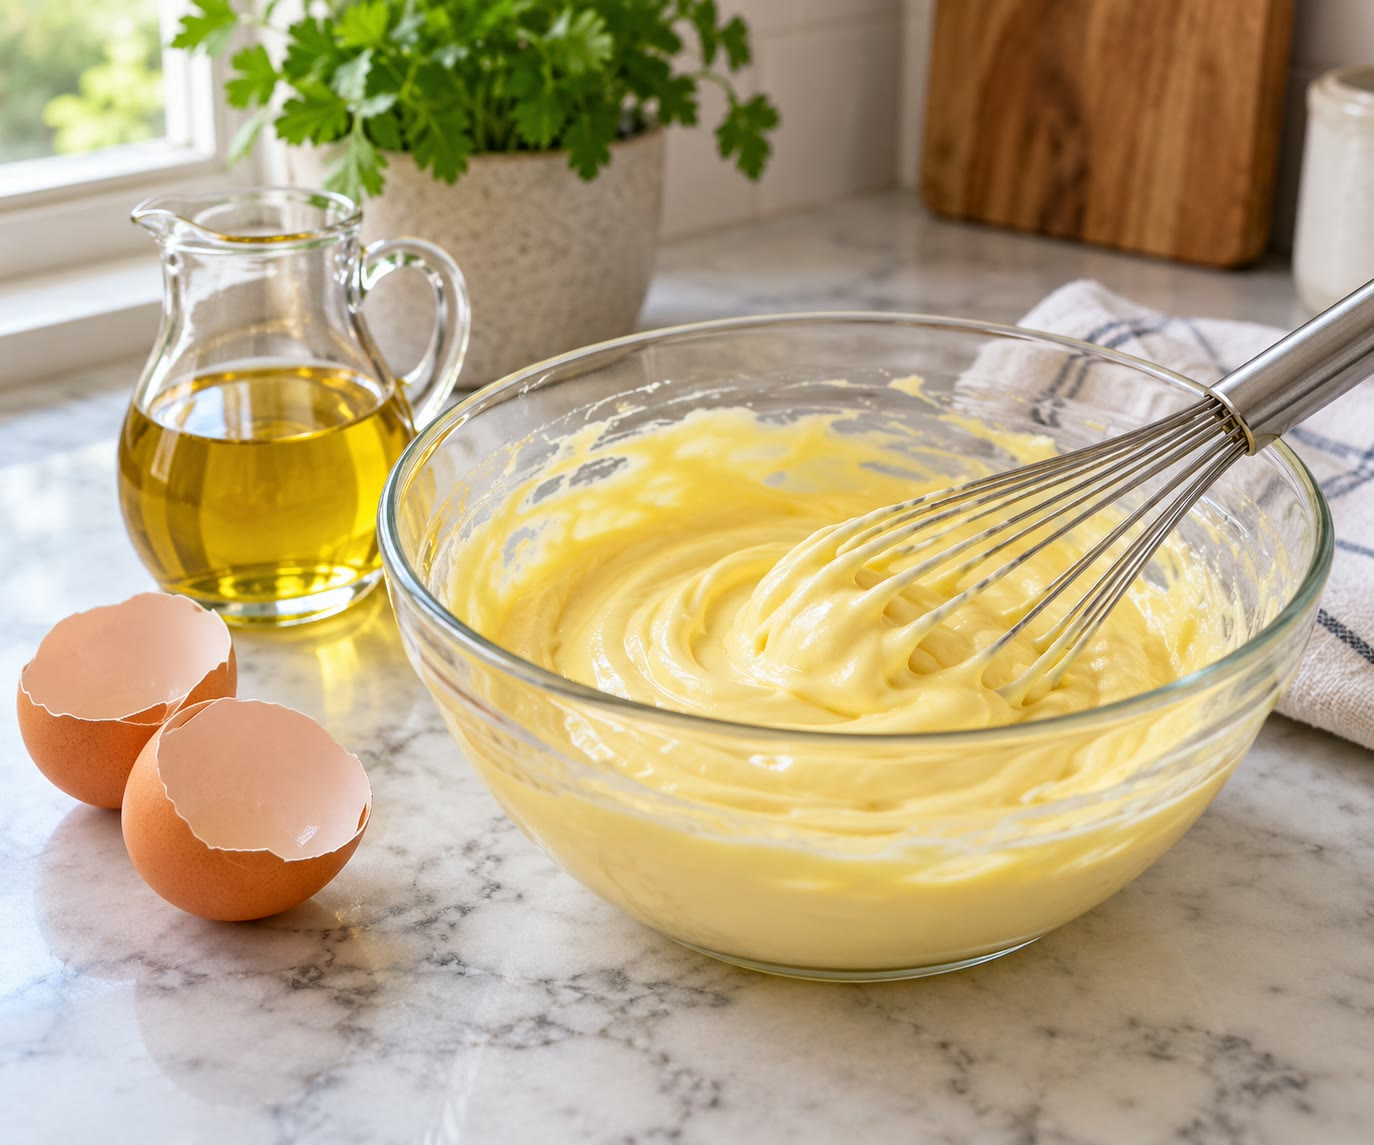
\includegraphics[width=0.6\linewidth]{images/book4/ai/b3-17-mayonnaise.jpg}

{\small फेंटा जा रहा मेयोनेज़: जल में तेल के बूँदकों का एक \omterm{def:b3:colloids:colloid}{पायस},
जो अंडे की ज़र्दी के \omterm{def:b3:colloids:surfactant}{पृष्ठसक्रियकों} से स्थायीकृत है।}
\end{omfigure}

\section{अंतरापृष्ठ और पृष्ठ तनाव}

किसी द्रव के स्थूल भाग में एक अणु सभी दिशाओं में समान रूप से आकर्षित होता है;
पृष्ठ पर वह अपने पड़ोसियों का एक भाग खो देता है। पृष्ठ बनाने में ऊर्जा लगती है।

\begin{definition}[पृष्ठ तनाव]\label{def:b3:colloids:surface-tension}
किसी द्रव का \emph{पृष्ठ तनाव}\index{पृष्ठ तनाव} $\gamma$ वह गिब्स
ऊर्जा है जो नियत ताप, दाब और संघटन पर उसके पृष्ठ का एकांक क्षेत्रफल बनाने के लिए
आवश्यक है: $\gamma = (\partial G/\partial A)_{T,p,n}$, \unit{J.m^{-2}} $=$ \unit{N.m^{-1}} में। दो प्रावस्थाओं के बीच के
अंतरापृष्ठ के लिए यह अंतरापृष्ठीय तनाव है।
\end{definition}

हाइड्रोजन आबंधों से बँधे जल का \omterm{def:b3:colloids:surface-tension}{पृष्ठ तनाव} ऊँचा है: \qty{25}{\celsius} पर \qty{72.0}{mN/m}।
ऐल्केनों का लगभग 20, पारे का लगभग 480 होता है।

\begin{proposition}[लाप्लास दाब]\label{prop:b3:colloids:laplace}
त्रिज्या $r$ की किसी गोलाकार बूँद या बुलबुले के भीतर का दाब बाहर के
दाब से इतना अधिक होता है:
\[
  \Delta p = \frac{2\gamma}{r} .
\]
\end{proposition}

\begin{proof}
साम्य पर त्रिज्या को $\dd r$ से बढ़ाइए: दाब-अंतर द्वारा किया गया
कार्य, $\Delta p\,4\pi r^2\dd r$, पृष्ठ गिब्स ऊर्जा की वृद्धि, $\gamma\,8\pi r\,\dd r$, के बराबर होता है।
\end{proof}

\begin{definition}[स्पर्श कोण, आर्द्रण]\label{def:b3:colloids:wetting}
किसी ठोस पर बूँद का \emph{स्पर्श कोण}\index{स्पर्श कोण} $\theta$ वह कोण है,
जो द्रव के भीतर से मापा जाता है, ठोस पृष्ठ और द्रव पृष्ठ के बीच,
उस रेखा पर जहाँ ठोस, द्रव और वाष्प मिलते हैं। कोई द्रव ठोस को \emph{आर्द्र करता है}\index{आर्द्रण}
जब $\theta < 90^\circ$, और पूर्णतः फैल जाता है जब $\theta = 0$।
\end{definition}

\begin{theorem}[यंग का समीकरण]\label{thm:b3:colloids:young}
साम्य पर तीनों अंतरापृष्ठीय तनाव और \omterm{def:b3:colloids:wetting}{स्पर्श कोण} यह संतुष्ट करते हैं
\[
  \gamma_{\mathrm{SV}} = \gamma_{\mathrm{SL}} + \gamma_{\mathrm{LV}}\cos\theta .
\]
यह \emph{यंग का समीकरण}\index{यंग का समीकरण} है।
\end{theorem}

\begin{proof}
स्पर्श रेखा को (रेखा की प्रति इकाई लंबाई) $\dd x$ से बाहर की ओर खिसकाइए: क्षेत्रफल $\dd x$
का ठोस--वाष्प अंतरापृष्ठ ठोस--द्रव अंतरापृष्ठ से प्रतिस्थापित होता है, और
द्रव--वाष्प अंतरापृष्ठ $\dd x\cos\theta$ से बढ़ता है। गिब्स ऊर्जा
$(\gamma_{\mathrm{SL}} - \gamma_{\mathrm{SV}} + \gamma_{\mathrm{LV}}\cos\theta)\dd x$ से बदलती है, जो साम्य पर शून्य है।
\end{proof}

\begin{omfigure}
\begin{tikzpicture}[font=\small, >=Stealth]
  \fill[black!12] (-3.6,-0.5) rectangle (3.6,0);
  \draw[thick] (-3.6,0) -- (3.6,0);
  \node[anchor=north] at (2.6,-0.05) {ठोस};
  \fill[omWater!60] (-2.0,0) arc[start angle=160, end angle=20, radius=2.13] -- cycle;
  \draw[thick, omDef] (-2.0,0) arc[start angle=160, end angle=20, radius=2.13];
  % circle centre 0.73 below the solid: a cap smaller than a hemisphere, contact angle 90 - 20 = 70 deg;
  % at the right contact point the liquid surface leaves at 110 deg (up and to the left)
  \draw[->, thick, omThm] (2.0,0) -- ++(110:1.3) node[anchor=south] {$\gamma_{\mathrm{LV}}$};
  \draw[->, thick] (2.0,0) -- (3.3,0) node[anchor=south] {$\gamma_{\mathrm{SV}}$};
  \draw[->, thick] (2.0,0) -- (0.7,0) node[anchor=north, yshift=-1pt] {$\gamma_{\mathrm{SL}}$};
  \draw (1.45,0) arc[start angle=180, end angle=110, radius=0.55];
  \node at (1.33,0.42) {$\theta$};
  \node at (0,0.6) {द्रव};
  \node at (-2.8,1.4) {वाष्प};
\end{tikzpicture}

{\small एक स्थिर बूँद और उसकी स्पर्श रेखा को खींचते तीन तनाव:
ठोस के अनुदिश उनके घटकों का संतुलन \omterm{thm:b3:colloids:young}{यंग का समीकरण} देता है; यहाँ $\theta
\approx 70^\circ$, एक आंशिक रूप से आर्द्रक द्रव।}
\end{omfigure}

\begin{theorem}[केल्विन समीकरण]\label{thm:b3:colloids:kelvin}
त्रिज्या $r$ की किसी गोलाकार बूँद का वाष्प दाब समतल
द्रव के वाष्प दाब, $p^*$, से अधिक होता है:
\[
  \ln\frac{p}{p^*} = \frac{2\gamma V_{\mathrm m}}{rRT},
\]
जहाँ $V_{\mathrm m}$ द्रव का मोलर आयतन है। यह \emph{केल्विन
समीकरण}\index{केल्विन समीकरण} है।
\end{theorem}

\begin{proof}
बूँद में द्रव अतिरिक्त दाब $2\gamma/r$ के अधीन है, जो उसका
रासायनिक विभव $V_{\mathrm m}\,2\gamma/r$ से बढ़ा देता है ($(\partial\mu/\partial p)_T = V_{\mathrm m}$ के साथ, द्रव को असंपीड्य मानकर)।
उसके साथ साम्य में वाष्प का रासायनिक विभव भी
उतना ही बढ़ना चाहिए: $RT\ln(p/p^*) = 2\gamma V_{\mathrm m}/r$।
\end{proof}

\qty{25}{\celsius} पर त्रिज्या \qty{10}{nm} के जल बूँदक के लिए $2\gamma V_{\mathrm m}/rRT = 0.105$: उसका वाष्प
दाब समतल जल से 11\,\% अधिक है। छोटे बूँदक वाष्पित होते हैं जबकि
बड़े बढ़ते हैं, और बादलों को आरंभ होने के लिए नाभिकों की आवश्यकता होती है; यही बात
छोटे क्रिस्टलों की विलेयता पर लागू होती है।

\begin{definition}[ओस्टवाल्ड परिपक्वन]\label{def:b3:colloids:ripening}
\emph{ओस्टवाल्ड परिपक्वन}\index{ओस्टवाल्ड परिपक्वन} किसी परिक्षेपण के बड़े
कणों या बूँदकों की छोटे कणों या बूँदकों की कीमत पर वृद्धि है,
जो छोटे कणों की उच्चतर विलेयता या वाष्प दाब से प्रेरित होती है।
\end{definition}

\section{पृष्ठसक्रियक और मिसेल}

\begin{definition}[पृष्ठसक्रियक]\label{def:b3:colloids:surfactant}
\emph{पृष्ठसक्रियक}\index{पृष्ठसक्रियक} (पृष्ठ-सक्रिय कारक) एक उभयरागी
अणु है जो अंतरापृष्ठों पर अधिशोषित होकर उनका तनाव घटाता है। यह
\emph{ऋणायनी पृष्ठसक्रियक}\index{ऋणायनी पृष्ठसक्रियक} है यदि इसका शीर्ष ऋणायन हो (सोडियम
डोडेसिल सल्फ़ेट, साबुन), \emph{धनायनी पृष्ठसक्रियक}\index{धनायनी पृष्ठसक्रियक}
यदि धनायन हो (चतुष्क अमोनियम लवण), और \emph{अनायनिक
पृष्ठसक्रियक}\index{अनायनिक पृष्ठसक्रियक} यदि शीर्ष एक उदासीन ध्रुवीय समूह हो (एथिलीन
ऑक्साइड इकाइयों की एक शृंखला)।
\end{definition}

\begin{definition}[पृष्ठ आधिक्य सांद्रता]\label{def:b3:colloids:surface-excess}
किसी विलेय की \emph{पृष्ठ आधिक्य सांद्रता}\index{पृष्ठ आधिक्य सांद्रता} $\Gamma$
अंतरापृष्ठ पर प्रति इकाई क्षेत्रफल विलेय की वह मात्रा है, जो उस मात्रा से अधिक है
जो उतना ही आयतन रखता यदि स्थूल सांद्रता ठीक अंतरापृष्ठ तक
बनी रहती।
\end{definition}

\begin{theorem}[गिब्स अधिशोषण समतापी]\label{thm:b3:colloids:gibbs-adsorption}
सांद्रता $c$ वाले किसी अनायनिक विलेय के तनु विलयन के लिए,
\[
  \Gamma = -\frac{1}{RT}\frac{\dd\gamma}{\dd\ln c};
\]
किसी 1:1 आयनिक \omterm{def:b3:colloids:surfactant}{पृष्ठसक्रियक} के लिए, बिना मिलाए गए लवण के, $RT$ के स्थान पर $2RT$ आता है। यह
\emph{गिब्स अधिशोषण समतापी}\index{गिब्स अधिशोषण समतापी} है।
\end{theorem}

\begin{proof}
अंतरापृष्ठ के लिए, नियत $T$ और
$p$ पर गिब्स--ड्यूहेम संबंध का अनुरूप $\dd\gamma = -\sum_i\Gamma_i\,\dd\mu_i$ है (पृष्ठ गिब्स ऊर्जा $\gamma A$, $G$ की भूमिका निभाती है,
स्वीकृत)। विभाजक पृष्ठ को इस प्रकार चुनने पर कि विलायक का कोई आधिक्य न हो,
$\dd\gamma = -\Gamma\,\dd\mu$, और तनु विलयन में $\dd\mu = RT\,\dd\ln c$। आयनिक \omterm{def:b3:colloids:surfactant}{पृष्ठसक्रियक} के लिए
धनायन और ऋणायन दोनों समान आधिक्य में अधिशोषित होते हैं और $\dd\mu$
$2RT\,\dd\ln c$ बन जाता है।
\end{proof}

जिस \omterm{def:b3:colloids:surfactant}{पृष्ठसक्रियक} का \omterm{def:b3:colloids:surface-tension}{पृष्ठ तनाव} $\ln c$ के साथ रैखिक रूप से गिरता है, उसका पृष्ठ आधिक्य
नियत होता है: अंतरापृष्ठ संतृप्त है, और $1/(\Gamma N_A)$ एक अधिशोषित अणु द्वारा
घेरा गया क्षेत्रफल है।

\begin{method}[$\gamma$--$\ln c$ ढलान से प्रति अणु क्षेत्रफल]\label{met:b3:colloids:surface-excess}
\begin{enumerate}
  \item CMC से नीचे $\gamma$ को $c$ के विरुद्ध मापिए; $\gamma$ को $\ln c$ के विरुद्ध आलेखित कीजिए।
  \item CMC से ठीक नीचे के रैखिक भाग का ढलान लीजिए; $\Gamma = -\text{ढलान}/(nRT)$, जहाँ \omterm{def:b3:colloids:surfactant}{अनायनिक पृष्ठसक्रियक} के लिए $n
        = 1$, और बिना लवण वाले 1:1 आयनिक के लिए 2।
  \item प्रति अणु क्षेत्रफल $= 1/(\Gamma N_A)$; विशिष्ट मान 0.3 से \qty{0.6}{nm^2} होते हैं।
\end{enumerate}
\end{method}

\begin{definition}[मिसेल, क्रांतिक मिसेल सांद्रता, समुच्चयन संख्या]\label{def:b3:colloids:micelle}
\emph{मिसेल}\index{मिसेल} विलयन में \omterm{def:b3:colloids:surfactant}{पृष्ठसक्रियक} अणुओं का एक समुच्चय है
जिसकी जलविरागी पुच्छें द्रव-सदृश क्रोड बनाती हैं, जिसे शीर्ष जल से
बचाए रखते हैं। \emph{क्रांतिक मिसेल सांद्रता}\index{क्रांतिक मिसेल सांद्रता}
(CMC) वह सांद्रता है जिसके ऊपर मिसेल बनते हैं; उनमें अणुओं की
माध्य संख्या \emph{समुच्चयन संख्या}\index{समुच्चयन संख्या} है।
\end{definition}

\begin{proposition}[CMC पर विराम]\label{prop:b3:colloids:cmc-break}
CMC से ऊपर मुक्त \omterm{def:b3:colloids:surfactant}{पृष्ठसक्रियक} की सांद्रता, और उसके साथ \omterm{def:b3:colloids:surface-tension}{पृष्ठ
तनाव} और परासरण दाब, लगभग नियत रहते हैं; मुक्त अणुओं पर निर्भर
गुणधर्म CMC पर अपना ढलान बदलते हैं।
\end{proposition}

\begin{proof}[आंशिक उपपत्ति]
\omterm{def:b3:colloids:micelle}{मिसेलों} को एक पृथक प्रावस्था मानिए: मिलाया गया \omterm{def:b3:colloids:surfactant}{पृष्ठसक्रियक} \omterm{def:b3:colloids:micelle}{मिसेलों} में तब जाता है जब
मुक्त अणुओं का रासायनिक विभव \omterm{def:b3:colloids:micelle}{मिसेल} में स्थित एक अणु के रासायनिक विभव तक पहुँच जाता है,
और तब यह रासायनिक विभव, अतः मुक्त सांद्रता, नियत
रहती है। \omterm{def:b3:colloids:surface-tension}{पृष्ठ तनाव}, जो गिब्स समतापी के माध्यम से मुक्त अणुओं द्वारा तय होता है, गिरना
बंद कर देता है; चालकता बढ़ती रहती है, पर अधिक धीरे, क्योंकि
\omterm{def:b3:colloids:micelle}{मिसेल} मुक्त आयनों की तुलना में प्रति \omterm{def:b3:colloids:surfactant}{पृष्ठसक्रियक} कम आवेश वहन करते हैं (उनके प्रति-आयनों का
एक भाग बँधा रहता है)। यह मॉडल एक सीमा है, क्योंकि परिमित आकार के \omterm{def:b3:colloids:micelle}{मिसेल}
सांद्रता के एक संकीर्ण परास पर बनते हैं (स्वीकृत)।
\end{proof}

\begin{method}[विराम से CMC]\label{met:b3:colloids:cmc}
\begin{enumerate}
  \item अपेक्षित CMC को समेटने वाले सांद्रता-परास पर \omterm{def:b3:colloids:surface-tension}{पृष्ठ तनाव} (या, आयनिक \omterm{def:b3:colloids:surfactant}{पृष्ठसक्रियक} के लिए,
        चालकता) मापिए।
  \item दोनों शाखाओं पर सीधी रेखाएँ समंजित कीजिए ($\gamma$, $\log c$ के विरुद्ध; या $\kappa$, $c$ के विरुद्ध)।
  \item उनका प्रतिच्छेदन CMC है।
\end{enumerate}
\end{method}

\begin{omfigure}
\begin{tikzpicture}
\begin{axis}[name=gm, width=0.47\linewidth, height=5.2cm, xmin=-5, xmax=-1.5, ymin=30, ymax=76,
  axis lines=left, xlabel={$\log(c/\unit{mol.L^{-1}})$}, ylabel={$\gamma$ / \unit{mN.m^{-1}}},
  tick label style={font=\small}, label style={font=\small}]
\addplot[omDef, very thick] table[x=logc, y=gamma_mN] {figdata/out/bachelor-3-surfactant-cmc-gamma.dat};
\draw[black!40, dashed] (axis cs:-2.086,30) -- (axis cs:-2.086,70);
\node[font=\scriptsize, anchor=south west] at (axis cs:-2.05,45) {CMC};
\end{axis}
\begin{axis}[at={(gm.east)}, anchor=west, xshift=1.4cm, width=0.47\linewidth, height=5.2cm,
  xmin=0, xmax=20, ymin=0, ymax=1.0, axis lines=left, xlabel={$c$ / mM},
  ylabel={$\kappa$ / \unit{mS.cm^{-1}}}, tick label style={font=\small}, label style={font=\small}]
\addplot[omThm, very thick] table[x=c_mM, y=kappa] {figdata/out/bachelor-3-surfactant-cmc-kappa.dat};
\draw[black!40, dashed] (axis cs:8.2,0) -- (axis cs:8.2,0.9);
\node[font=\scriptsize, anchor=south west] at (axis cs:8.4,0.15) {CMC};
\end{axis}
\end{tikzpicture}

{\small सोडियम डोडेसिल सल्फ़ेट की CMC वाला एक मॉडल आयनिक \omterm{def:b3:colloids:surfactant}{पृष्ठसक्रियक},
\qty{25}{\celsius} पर \qty{8.2}{mM}। बाएँ: \omterm{def:b3:colloids:surface-tension}{पृष्ठ तनाव} $\log c$ के साथ गिरता है, CMC से ठीक नीचे
रैखिक रूप से (एक संतृप्त अंतरापृष्ठ, प्रति अणु लगभग \qty{0.6}{nm^2} क्षेत्रफल), फिर
नियत रहता है। दाएँ: CMC से ऊपर चालकता कम तीव्रता से बढ़ती है।}
\end{omfigure}

\begin{definition}[संकुलन प्राचल]\label{def:b3:colloids:packing}
किसी \omterm{def:b3:colloids:surfactant}{पृष्ठसक्रियक} का \emph{संकुलन प्राचल}\index{संकुलन प्राचल} $P =
v/(a_0l)$ है, जहाँ $v$ उसकी जलविरागी पुच्छ का आयतन है, $l$ फैली हुई पुच्छ की
लंबाई और $a_0$ समुच्चय के पृष्ठ पर प्रति शीर्ष समूह इष्टतम क्षेत्रफल।
\end{definition}

\begin{proposition}[समुच्चयों की आकृति]\label{prop:b3:colloids:packing}
गोलीय \omterm{def:b3:colloids:micelle}{मिसेलों} के लिए $P \le \frac13$, बेलनाकार \omterm{def:b3:colloids:micelle}{मिसेलों} के लिए $\frac13 < P \le \frac12$, समतल द्विपरतों
(पुटिकाएँ, झिल्लियाँ) के लिए $\frac12 < P \le 1$ आवश्यक है; $P > 1$ उलटी संरचनाएँ देता है।
\end{proposition}

\begin{proof}
त्रिज्या $R \le l$ के एक गोले में, जो $N$ अणुओं से बना है, $Nv = \frac43\pi R^3$ और $Na_0 = 4\pi R^2$, अतः
$v/a_0 = R/3 \le l/3$: $P \le \frac13$। त्रिज्या $R$ और लंबाई $L$ के बेलन के लिए $Nv = \pi R^2L$ और
$Na_0 = 2\pi RL$: $v/a_0 = R/2 \le l/2$। मोटाई $2l$ और क्षेत्रफल $A$ की द्विपरत के लिए $Nv = 2lA$ और
$Na_0 = 2A$: $v/a_0 = l$।
\end{proof}

\begin{omfigure}
\begin{tikzpicture}[font=\scriptsize]
  % a sphere-forming cone
  \draw[omDef, thick, fill=omDef!15] (0,0) -- (-0.45,1.2) arc[start angle=180, end angle=0, radius=0.45] -- cycle;
  \node at (0,-0.3) {$P < \frac13$: शंकु};
  % micelle
  \begin{scope}[xshift=2.2cm, yshift=0.6cm]
    \foreach \a in {0,30,...,330}{\draw[black!60] (\a:0.2) -- (\a:0.62); \fill[omDef] (\a:0.7) circle (0.09);}
    \node at (0,-1.05) {गोलीय मिसेल};
  \end{scope}
  % truncated cone
  \begin{scope}[xshift=4.7cm]
    \draw[omDef, thick, fill=omDef!15] (-0.18,0) -- (-0.4,1.2) -- (0.4,1.2) -- (0.18,0) -- cycle;
    \node at (0,-0.3) {$\frac13 < P < \frac12$};
  \end{scope}
  \begin{scope}[xshift=6.9cm, yshift=0.6cm]
    \fill[omDef!10] (-0.9,-0.55) rectangle (0.9,0.55);
    \foreach \x in {-0.8,-0.5,...,0.8}{\fill[omDef] (\x,0.62) circle (0.08); \fill[omDef] (\x,-0.62) circle (0.08);}
    \node at (0,-1.05) {बेलन (पार्श्व दृश्य)};
  \end{scope}
  % cylinder shape
  \begin{scope}[xshift=9.4cm]
    \draw[omDef, thick, fill=omDef!15] (-0.3,0) rectangle (0.3,1.2);
    \node at (0,-0.3) {$P \approx 1$: बेलन};
  \end{scope}
  \begin{scope}[xshift=11.4cm, yshift=0.6cm]
    \foreach \x in {-0.8,-0.6,...,0.8}{
      \draw[black!60] (\x,0.5) -- (\x,0.05) (\x,-0.5) -- (\x,-0.05);
      \fill[omDef] (\x,0.58) circle (0.08); \fill[omDef] (\x,-0.58) circle (0.08);}
    \node at (0,-1.05) {द्विपरत};
  \end{scope}
\end{tikzpicture}

{\small आण्विक आकृति और समुच्चय की आकृति। बड़े शीर्ष और
एक पुच्छ वाला \omterm{def:b3:colloids:surfactant}{पृष्ठसक्रियक} (एक शंकु) गोलीय \omterm{def:b3:colloids:micelle}{मिसेलों} में संकुलित होता है; छोटे शीर्ष वाला
बेलनों में; पुच्छ पर उतना ही चौड़ा जितना शीर्ष पर, जैसे दो शृंखलाओं वाला
लिपिड, समतल द्विपरतों में, जो पुटिकाओं और कोशिका झिल्लियों की दीवारें हैं।}
\end{omfigure}

अपमार्जन इन प्रभावों को जोड़ता है: \omterm{def:b3:colloids:surfactant}{पृष्ठसक्रियक} जल और किसी तैलीय मैल के बीच
अंतरापृष्ठीय तनाव को तब तक घटाता है जब तक मैल लुढ़ककर बूँदों में न बदल जाए,
जिन्हें फिर \omterm{def:b3:colloids:micelle}{मिसेल} अपने क्रोड में विलेयित कर लेते हैं।

\section{कोलॉइड}

\begin{definition}[कोलॉइड]\label{def:b3:colloids:colloid}
\emph{कोलॉइड}\index{कोलॉइड} लगभग \qty{1}{nm} से \qty{1}{\micro m} चौड़े कणों, बूँदकों या बुलबुलों
(\emph{परिक्षिप्त प्रावस्था}\index{परिक्षिप्त प्रावस्था})
का एक सतत \emph{परिक्षेपण माध्यम}\index{परिक्षेपण माध्यम} में परिक्षेपण है।
\emph{सॉल}\index{सॉल} किसी द्रव में ठोस कणों का परिक्षेपण है,
\emph{पायस}\index{पायस} किसी अन्य द्रव में द्रव बूँदकों का,
\emph{फेन}\index{फेन} किसी द्रव या ठोस में गैस बुलबुलों का, \emph{जेल}\index{जेल}
कणों या बहुलकों का एक जाल जो पूरे द्रव में फैलकर उसे
ठोस-सदृश बना देता है, और \emph{एरोसॉल}\index{एरोसॉल} किसी गैस में बूँदकों या कणों का परिक्षेपण।
\end{definition}

कोलॉइडी कण इतने छोटे होते हैं कि ब्राउनी गति (विलायक अणुओं के
यादृच्छिक धक्के, भौतिकी से) द्वारा निलंबित रह सकें, और इतने बड़े कि प्रकाश
प्रकीर्णित कर सकें।

\begin{definition}[टिंडल प्रभाव]\label{def:b3:colloids:tyndall}
\emph{टिंडल प्रभाव}\index{टिंडल प्रभाव} किसी \omterm{def:b3:colloids:colloid}{कोलॉइड} के कणों द्वारा प्रकाश का
प्रकीर्णन है, जिससे \omterm{def:b3:colloids:colloid}{कोलॉइड} से गुज़रता हुआ प्रकाश-पुंज पार्श्व से दिखाई देने
लगता है, जबकि एक वास्तविक विलयन अदृश्य रहता है।
\end{definition}

\begin{omfigure}
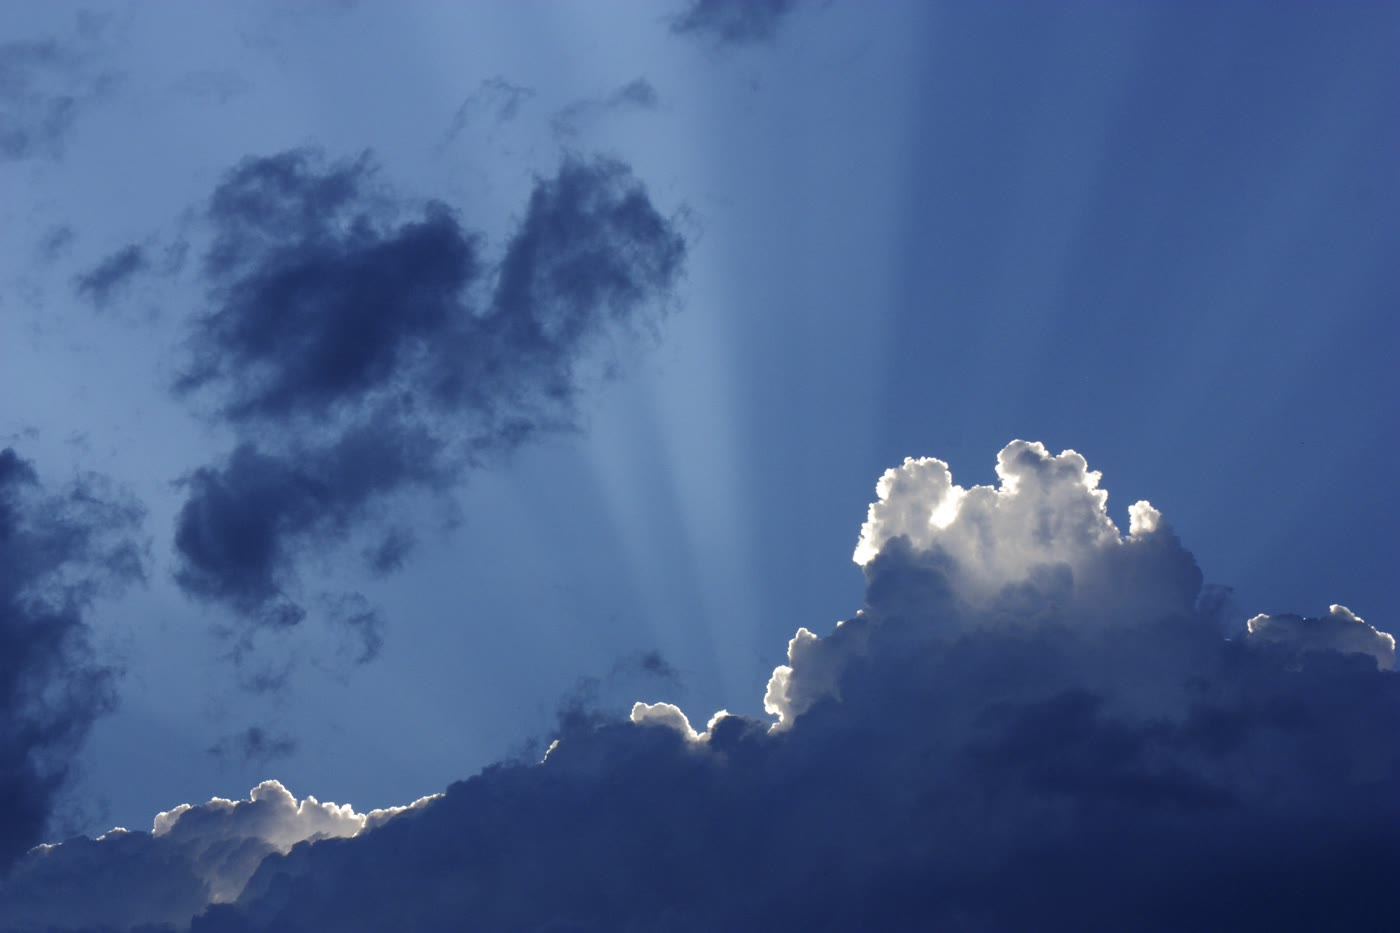
\includegraphics[width=0.55\linewidth]{images/book4/tyndall-sky.jpg}

{\small बादलों की एक दरार से आती सूर्य-किरणें: वे इसलिए दिखाई देती हैं कि
वायु का \omterm{def:b3:colloids:colloid}{एरोसॉल}, बूँदक और धूल, प्रकाश के एक भाग को पार्श्व में प्रकीर्णित करता है;
आकाश के पैमाने पर \omterm{def:b3:colloids:tyndall}{टिंडल प्रभाव}।}
\end{omfigure}

\section{कोलॉइडी स्थायित्व}

दो कोलॉइडी कण लघु परास पर वान्डरवाल्स बलों द्वारा सदैव
एक-दूसरे को आकर्षित करते हैं। जल में अधिकांश कणों पर आवेश भी होता है (आयनित पृष्ठ
समूह, अधिशोषित आयन), जो प्रति-आयनों की एक \omterm{def:b3:electrode-kinetics:double-layer}{विसरित परत} से घिरा होता है:
\cref{ch:b3:electrode-kinetics} की द्विपरत। जब दो कण पास आते हैं, तो उनकी
\omterm{def:b3:electrode-kinetics:double-layer}{विसरित परतें} अतिव्याप्त होकर प्रतिकर्षण करती हैं।

\begin{definition}[ज़ीटा विभव]\label{def:b3:colloids:zeta}
किसी कण का \emph{ज़ीटा विभव}\index{ज़ीटा विभव} $\zeta$ उसके सर्पण तल पर वैद्युत
विभव है, जो द्विपरत के भीतर कण के साथ गति करने वाले द्रव और
गति न करने वाले द्रव के बीच की सीमा है; इसे विद्युत क्षेत्र में कणों के वेग
(वैद्युतकणसंचलन) से मापा जाता है।
\end{definition}

\begin{omfigure}
\begin{tikzpicture}[font=\scriptsize]
  \fill[black!20] (0,0) circle (1.2);
  \foreach \a in {0,30,...,330}{\node at (\a:1.05) {$-$};}
  \draw[omDef, dashed] (0,0) circle (1.55);
  \foreach \a in {15,45,...,345}{\draw[omDef, fill=omDef!15] (\a:1.38) circle (0.11); \node at (\a:1.38) {\tiny$+$};}
  \draw[omThm, thick, densely dotted] (0,0) circle (1.85);
  \foreach \a/\r/\s in {10/2.2/+, 50/2.5/+, 95/2.3/-, 130/2.7/+, 175/2.2/+, 215/2.6/-, 250/2.3/+, 290/2.8/+, 345/2.6/+}{
    \draw[black!60, fill=white] (\a:\r) circle (0.11); \node at (\a:\r) {\tiny$\s$};}
  \draw[->, black!60] (2.6,1.6) node[anchor=west] {स्टर्न परत} -- (40:1.6);
  \draw[->, omThm] (2.6,-1.4) node[anchor=west] {सर्पण तल: $\zeta$} -- (-30:1.87);
  \node at (0,0) {कण};
  \node[anchor=west] at (2.9,0.2) {विसरित परत};
\end{tikzpicture}

{\small अपनी द्विपरत सहित एक ऋणावेशित कण: प्रति-आयनों की एक संहत स्टर्न
परत, उसके ठीक आगे सर्पण तल, जहाँ \omterm{def:b3:colloids:zeta}{ज़ीटा
विभव} परिभाषित है, और \omterm{def:b3:electrode-kinetics:double-layer}{विसरित परत}, जिसमें कुछ डिबाई लंबाइयों तक प्रति-आयन
सह-आयनों से अधिक होते हैं।}
\end{omfigure}

\begin{theorem}[DLVO सिद्धांत]\label{thm:b3:colloids:dlvo}
त्रिज्या $a$ के दो गोलों के लिए, जो अंतराल $h \ll a$ से पृथक हैं, विसरित-परत विभव
$\psi$ और हमाकर स्थिरांक $A$ के साथ, निम्न विभवों पर अन्योन्यक्रिया ऊर्जा है
\[
  V(h) = 2\pi\varepsilon_r\varepsilon_0a\psi^2\ln\bigl(1 + \eu^{-\kappa h}\bigr) - \frac{Aa}{12h} .
\]
पहला पद, द्विपरत प्रतिकर्षण, \omterm{def:b3:electrode-kinetics:double-layer}{डिबाई लंबाई} $\kappa^{-1}$ पर क्षयित होता है;
दूसरा, वान्डरवाल्स आकर्षण, लवण पर निर्भर नहीं करता। उनके योग में
लवण सांद्रता कम होने पर कुछ डिबाई लंबाइयों पर एक ऊर्जा अवरोध होता है,
और एक क्रांतिक सांद्रता से ऊपर कोई अवरोध नहीं।
\end{theorem}

\begin{proof}[आंशिक उपपत्ति]
दोनों रूप स्वीकृत हैं (प्रतिकर्षण, देर्यागिन सन्निकटन में दो गूई--चैपमैन
परतों के अतिव्यापन से; आकर्षण, दोनों पिंडों पर लंदन
अन्योन्यक्रियाओं के योग से)। आयनिक सामर्थ्य बढ़ाने से $\kappa$ बढ़ता है
(\cref{prop:b3:electrode-kinetics:debye-length}): तब प्रतिकर्षण
छोटे $h$ पर समाप्त हो जाता है, जहाँ आकर्षण, जो $1/h$ के अनुसार बढ़ता है, प्रबलतर है;
$V$ का अधिकतम घटता है और अंततः लुप्त हो जाता है।
\end{proof}

\begin{omfigure}
\begin{tikzpicture}
\begin{axis}[width=0.72\linewidth, height=5.6cm, xmin=0, xmax=30, ymin=-40, ymax=45,
  axis lines=left, xlabel={अंतराल $h$ / nm}, ylabel={$V/kT$},
  tick label style={font=\small}, label style={font=\small},
  legend style={font=\scriptsize, draw=none, at={(0.98,0.98)}, anchor=north east}, legend cell align=left]
\addplot[omDef, thick] table[x=h_nm, y=I1] {figdata/out/bachelor-3-dlvo.dat};
\addplot[black!60, thick] table[x=h_nm, y=I10] {figdata/out/bachelor-3-dlvo.dat};
\addplot[omThm, thick] table[x=h_nm, y=I50] {figdata/out/bachelor-3-dlvo.dat};
\addplot[black, thick, dashed] table[x=h_nm, y=I200] {figdata/out/bachelor-3-dlvo.dat};
\draw[black!30] (axis cs:0,0) -- (axis cs:30,0);
\legend{\qty{1}{mM}, \qty{10}{mM}, \qty{50}{mM}, \qty{200}{mM}}
\end{axis}
\end{tikzpicture}

{\small त्रिज्या \qty{100}{nm} के दो कणों की DLVO अन्योन्यक्रिया (मॉडल: विसरित-परत
विभव \qty{-30}{mV}, हमाकर स्थिरांक \qty{2e-20}{J}), 1:1 लवण वाले जल में। \qty{1}{mM} पर
लगभग $40\,kT$ का अवरोध कणों को अलग रखता है; \qty{10}{mM} पर यह आधा हो जाता है;
लगभग \qty{50}{mM} पर यह लुप्त हो जाता है और हर संघट्ट चिपकाने वाला होता है।}
\end{omfigure}

\begin{definition}[स्कंदन और स्थायीकरण]\label{def:b3:colloids:stability}
\emph{स्कंदन}\index{स्कंदन} कोलॉइडी कणों का वह समुच्चयन है जो उनके
स्थिरवैद्युत प्रतिकर्षण के लोप से होता है; \emph{ऊर्णन}\index{ऊर्णन}
ढीले ऊर्णों में समुच्चयन है, जो प्रायः अधिशोषित बहुलकों द्वारा जुड़े होते हैं।
किसी विद्युत-अपघट्य की \emph{क्रांतिक स्कंदन सांद्रता}\index{क्रांतिक स्कंदन सांद्रता}
(CCC) वह सांद्रता है जिसके ऊपर कोई
\omterm{def:b3:colloids:colloid}{कोलॉइड} तेज़ी से स्कंदित होता है। \emph{त्रिविम स्थायीकरण}\index{त्रिविम स्थायीकरण}
अधिशोषित या प्रत्यारोपित बहुलक शृंखलाओं द्वारा कणों को अलग रखता है,
जिनके अतिव्यापन में एन्ट्रॉपी की हानि होती।
\end{definition}

\begin{proposition}[शुल्त्से--हार्डी नियम]\label{prop:b3:colloids:schulze-hardy}
किसी अत्यधिक आवेशित \omterm{def:b3:colloids:colloid}{कोलॉइड} के लिए, किसी विद्युत-अपघट्य की \omterm{def:b3:colloids:stability}{क्रांतिक स्कंदन सांद्रता}
उसके प्रति-आयनों के आवेश $z$ की छठी घात के व्युत्क्रम के अनुसार बदलती है:
$\text{CCC} \propto z^{-6}$, अनुपात $1 : \frac{1}{64} : \frac{1}{729}$ में, $z = 1, 2, 3$ के लिए।
\end{proposition}

\begin{proof}[आंशिक उपपत्ति]
\emergencystretch=3em दो समतल प्लेटें लीजिए। उच्च पृष्ठ विभव पर प्रति इकाई क्षेत्रफल द्विपरत प्रतिकर्षण
$V_R = (64nkT/\kappa)\eu^{-\kappa h}$ की ओर प्रवृत्त होता है, जहाँ $n$, $z{:}z$
विद्युत-अपघट्य का संख्या घनत्व है, विभव से स्वतंत्र (स्वीकृत); आकर्षण $V_A =
-A/(12\pi h^2)$ है। CCC पर अवरोध ठीक लुप्त होता है: एक ही अंतराल पर $V = 0$ और $\dd V/\dd h = 0$।
चूँकि $\dd V_R/\dd h = -\kappa V_R$ और $\dd V_A/\dd h = -2V_A/h$, दोनों शर्तें देती हैं
$\kappa V_R = 2V_R/h$, अतः $\kappa h = 2$, और फिर $64nkT\eu^{-2}/\kappa = A\kappa^2/(48\pi)$, अर्थात् $n \propto \kappa^3$।
$\kappa^2 = 2nz^2e^2/(\varepsilon kT)$ के साथ, $\kappa^3 \propto (nz^2)^{3/2}$ और $n \propto n^{3/2}z^3$: अतः $n \propto z^{-6}$।
\end{proof}

\begin{omfigure}
\begin{tikzpicture}[font=\small, >=Stealth]
  \foreach \x/\lab/\v in {0/\ce{Na+}/1, 2.6/\ce{Ca^{2+}}/{1/64}, 5.2/\ce{Al^{3+}}/{1/729}}{
    \node at (\x,0) {\lab};
    \node[font=\scriptsize] at (\x,-0.45) {CCC $\times\,\v$};}
  \draw[->, thick, omDef] (-0.8,-0.95) -- (6.0,-0.95) node[midway, below, font=\scriptsize] {ऋणात्मक कोलॉइड के स्कंदन के लिए कम मात्रा};
\end{tikzpicture}

{\small ऋणावेशित \omterm{def:b3:colloids:colloid}{कोलॉइड} के लिए शुल्त्से--हार्डी नियम: \omterm{def:b3:colloids:stability}{क्रांतिक
स्कंदन सांद्रता} प्रति-आयन आवेश की छठी घात के अनुसार गिरती है।}
\end{omfigure}

यह नियम बताता है कि ऐलुमिनियम लवण जल को स्वच्छ करने में इतने प्रभावी क्यों हैं, और
नदियाँ समुद्र के लवणीय जल से मिलने के स्थान पर अपनी मृदा का भार क्यों छोड़ देती हैं।

\begin{method}[स्कंदक मात्रा का चयन]\label{met:b3:colloids:coagulant-dose}
\begin{enumerate}
  \item निलंबन के लिए किसी संदर्भ विद्युत-अपघट्य की CCC मापिए (बढ़ती मात्राओं के साथ
        जार परीक्षण, बैठने का प्रेक्षण करते हुए)।
  \item शुल्त्से--हार्डी नियम से इसे स्कंदक के प्रति-आयन के अनुसार मापित कीजिए।
  \item सूत्र की सहायता से इसे प्रति घन मीटर लवण के द्रव्यमान में बदलिए; जल-अपघटन
        और उससे उपभुक्त क्षारीयता के लिए पर्याप्त अतिरिक्त मिलाइए।
  \item अतिमात्रा से बचिए: अत्यधिक आवेशित प्रति-आयन कणों के आवेश का चिह्न
        उलटकर उन्हें पुनः स्थायी बना सकते हैं।
\end{enumerate}
\end{method}

\section{कार्यरत कोलॉइड}

\begin{definition}[जलरागी--वसारागी संतुलन]\label{def:b3:colloids:hlb}
किसी \omterm{def:b3:colloids:surfactant}{अनायनिक पृष्ठसक्रियक} का \emph{जलरागी--वसारागी संतुलन}\index{जलरागी--वसारागी संतुलन}
(HLB), ग्रिफ़िन के पैमाने पर, उसके जलरागी भाग के द्रव्यमान अंश का $20$
गुना है: निम्न मान (3 से 6) जल-में-तेल
\omterm{def:b3:colloids:colloid}{पायसों} के लिए उपयुक्त हैं, उच्च मान (8 से 18) तेल-में-जल \omterm{def:b3:colloids:colloid}{पायसों} और अपमार्जकों के लिए।
\end{definition}

\omterm{def:b3:colloids:colloid}{पायस} ऊष्मागतिकीय रूप से अस्थायी होते हैं, क्योंकि हर बूँदक
अंतरापृष्ठीय ऊर्जा वहन करता है; पायसीकारक उस ऊर्जा को घटाकर और हर बूँदक के चारों ओर
एक प्रतिकर्षी परत, आवेशित या त्रिविम, जोड़कर उन्हें गतिकतः स्थायी बनाते हैं।
मेयोनेज़ तेल-में-जल \omterm{def:b3:colloids:colloid}{पायस} है जिसमें इतना अधिक तेल (आयतन का लगभग चार-पाँचवाँ भाग)
होता है कि बूँदक एक-दूसरे से दबे रहते हैं, जिससे यह
एक मृदु ठोस बन जाता है। \omterm{def:b3:colloids:colloid}{फेन} ऐसे \omterm{def:b3:colloids:surfactant}{पृष्ठसक्रियकों} द्वारा स्थायीकृत होते हैं जो बुलबुलों के बीच की
द्रव फ़िल्मों के रिसाव को धीमा करते हैं; फेनरोधी, प्रायः सिलिकोन तेल, उन
फ़िल्मों पर फैलकर उन्हें तोड़ देते हैं। पेयजल संयंत्रों में ऐलुमिनियम या आयरन(III) लवण
उन मृदा और कार्बनिक \omterm{def:b3:colloids:colloid}{कोलॉइडों} को स्कंदित करते हैं जो नदी के जल को गंदला बनाते हैं; उनसे बना
हाइड्रॉक्साइड बैठते हुए ऊर्णों को नीचे बहा ले जाता है। धातु नैनोकण
अधिशोषित सिट्रेट आयनों (स्थिरवैद्युत) या थायोल-बद्ध
बहुलक शृंखलाओं (त्रिविम) द्वारा परिक्षिप्त रखे जाते हैं।

\begin{inthelab}[द्यू नूई वलय]
प्लैटिनम का एक वलय, जिसे साफ़ करने के लिए ज्वाला में तपाया गया हो, एक तुला से लटकाया जाता है और
द्रव में क्षैतिज रूप से डुबोया जाता है, फिर धीरे-धीरे ऊपर उठाया जाता है। उसे पृष्ठ से
खींचने के लिए आवश्यक बल एक अधिकतम से गुज़रता है; वलय की परिधि के दुगुने से
भाग देकर और उठे हुए नवचंद्रक की आकृति के लिए संशोधित करके, यह
\omterm{def:b3:colloids:surface-tension}{पृष्ठ तनाव} देता है। किसी \omterm{def:b3:colloids:surfactant}{पृष्ठसक्रियक} श्रेणी का मापन सबसे
तनु विलयन से आरंभ होता है, और नमूनों के बीच वलय को धोया जाता है।
\end{inthelab}

\begin{safety}{\ghs[0.8cm]{GHS02}\ghs[0.8cm]{GHS05}\ghs[0.8cm]{GHS07}}
% ledger: ghs4:SDS, ghs4:Al2SO43
सोडियम डोडेसिल सल्फ़ेट चूर्ण: ज्वलनशील ठोस, निगलने पर हानिकारक, आँखों को
गंभीर क्षति पहुँचाता है, श्वसन मार्ग में जलन करता है; धूल उठाए बिना,
नेत्र-सुरक्षा के साथ तौला जाता है। ऐलुमिनियम सल्फ़ेट (\ghs[0.6cm]{GHS05}): आँखों को गंभीर
क्षति पहुँचाता है।
\end{safety}

\begin{history}[टिंडल और अतिसूक्ष्मदर्शी]
जॉन टिंडल ने 1869 में दिखाया कि सूक्ष्म कणों से लदी वायु में प्रकाश-पुंज
दिखाई देने लगता है और उनसे मुक्त वायु में अदृश्य रहता है, तथा प्रकीर्णित
प्रकाश नीलाभ और ध्रुवित होता है। रिचर्ड ज़िग्मोंडी ने स्वर्ण \omterm{def:b3:colloids:colloid}{सॉलों} के लाल रंग
का अध्ययन करते हुए 1903 में हेनरी ज़ीडेनटॉप्फ़ के साथ अतिसूक्ष्मदर्शी बनाया, जो
\omterm{def:b3:colloids:colloid}{कोलॉइड} को पार्श्व से प्रकाशित करता है और प्रत्येक कण को अँधेरी पृष्ठभूमि पर
प्रकीर्णित प्रकाश के एक बिंदु के रूप में दिखाता है, विभेदित होने के लिए बहुत छोटा, पर गिनने योग्य।
\omterm{def:b3:colloids:colloid}{कोलॉइडों} पर अपने कार्य के लिए उन्हें रसायन का 1925 का नोबेल पुरस्कार मिला।
\end{history}

\section{अभ्यास}

\begin{exercise}[$\star$]\label{exo:b3:colloids:1}
% ledger: st:H2O.25C
\qty{25}{\celsius} पर जल में \qty{1.0}{\micro m} व्यास के एक वायु बुलबुले के भीतर का दाब
परिकलित कीजिए (बाहर: \qty{1.0}{bar})।
\end{exercise}

\begin{exercise}[$\star$]\label{exo:b3:colloids:2}
% ledger: st:H2O.25C
\qty{25}{\celsius} पर समतल जल के सापेक्ष त्रिज्या \qty{10}{nm} के जल बूँदक का वाष्प दाब
परिकलित कीजिए ($V_{\mathrm m} = \qty{18.07}{cm^3/mol}$)।
\end{exercise}

\begin{exercise}[$\star$]\label{exo:b3:colloids:3}
$\gamma_{\mathrm{LV}} = \qty{72}{mN/m}$ वाला एक द्रव, $\gamma_{\mathrm{SV}} = \qty{40}{mN/m}$ और $\gamma_{\mathrm{SL}} =
\qty{20}{mN/m}$ वाले ठोस पर (अभ्यास के आँकड़े): \omterm{def:b3:colloids:wetting}{स्पर्श कोण} परिकलित कीजिए। क्या यह \omterm{def:b3:colloids:wetting}{आर्द्र करता है}?
\end{exercise}

\begin{exercise}[$\star$]\label{exo:b3:colloids:4}
% ledger: eps:H2O.25C
\qty{25}{\celsius} पर जल में NaCl के और \ce{MgSO4} के \qty{0.010}{mol/L} के लिए \omterm{def:b3:electrode-kinetics:double-layer}{डिबाई लंबाई}
परिकलित कीजिए।
\end{exercise}

\begin{exercise}[$\star\star$]\label{exo:b3:colloids:5}
अपनी CMC से ठीक नीचे, एक आयनिक \omterm{def:b3:colloids:surfactant}{पृष्ठसक्रियक} (1:1, बिना लवण) का \omterm{def:b3:colloids:surface-tension}{पृष्ठ तनाव}
\qty{25}{\celsius} पर $\ln c$ की प्रति इकाई \qty{12.6}{mN/m} गिरता है। पृष्ठ आधिक्य और
प्रति अणु क्षेत्रफल परिकलित कीजिए।
\end{exercise}

\begin{exercise}[$\star\star$]\label{exo:b3:colloids:6}
एक \omterm{def:b3:colloids:surfactant}{अनायनिक पृष्ठसक्रियक} के \omterm{def:b3:colloids:surface-tension}{पृष्ठ तनाव}: $\log c = -5.0$, $-4.5$, $-4.0$, $-3.5$, $-3.0$ और $-2.5$ पर
52.0, 45.5, 39.1, 33.4, 33.3 और \qty{33.4}{mN/m} (अभ्यास के आँकड़े)।
CMC का आकलन कीजिए।
\end{exercise}

\begin{exercise}[$\star\star$]\label{exo:b3:colloids:7}
सोडियम डोडेसिल सल्फ़ेट के लिए $v = \qty{0.350}{nm^3}$, $l = \qty{1.67}{nm}$ और $a_0 = \qty{0.60}{nm^2}$ लीजिए; ऐसी
दो शृंखलाओं वाले लिपिड के लिए $2v$, वही $l$ और $a_0 = \qty{0.65}{nm^2}$ (अभ्यास के
आँकड़े)। उनके समुच्चयों की आकृति का पूर्वानुमान कीजिए।
\end{exercise}

\begin{exercise}[$\star\star$]\label{exo:b3:colloids:8}
एक ऋणावेशित \omterm{def:b3:colloids:colloid}{सॉल} \qty{60}{mM} NaCl पर स्कंदित होता है। \ce{CaCl2}
और \ce{AlCl3} के साथ CCC का पूर्वानुमान कीजिए। \ce{Na3PO4} क्या करेगा?
\end{exercise}

\begin{exercise}[$\star\star$]\label{exo:b3:colloids:9}
% ledger: cmc:C12E6
हेक्साएथिलीन ग्लाइकॉल मोनोडोडेसिल ईथर,
\ce{C12H25(OCH2CH2)6OH}, जिसका जलरागी भाग $\ce{(OCH2CH2)6OH}$ है, का ग्रिफ़िन HLB परिकलित कीजिए। क्या यह
तेल-में-जल \omterm{def:b3:colloids:colloid}{पायस} के लिए उपयुक्त है?
\end{exercise}

\begin{exercise}[$\star\star\star$]\label{exo:b3:colloids:10}
एक परिक्षेपण में 50 और \qty{500}{nm} त्रिज्या के बूँदक हैं। विलेयता पर लागू \omterm{thm:b3:colloids:kelvin}{केल्विन
समीकरण} का उपयोग करके समझाइए कि कौन बढ़ते हैं और कौन सिकुड़ते हैं, और
\omterm{def:b3:colloids:colloid}{पायस} संगलन के बिना भी समय के साथ स्थूल क्यों होते जाते हैं।
\end{exercise}

\begin{exercise}[$\star\star\star$]\label{exo:b3:colloids:11}
लाप्लास दाब से दिखाइए कि द्रव ऊँचाई $h = 2\gamma\cos\theta/(\rho gr)$ तक चढ़ता है,
त्रिज्या $r$ की केशिका में, और जल के लिए ($\theta = 0$, \qty{0.10}{mm} त्रिज्या) इसकी गणना कीजिए।
\end{exercise}

\begin{exercise}[$\star\star\star$]\label{exo:b3:colloids:12}
DLVO चित्र का उपयोग करके समझाइए कि \qty{1}{mM} पर स्थायी \omterm{def:b3:colloids:colloid}{सॉल} में \qty{100}{mM} NaCl मिलाने से
वह स्कंदित क्यों हो जाता है, जबकि कोई अनधिशोषी बहुलक मिलाने से
अवरोध नहीं बदलता, पर कणों पर प्रत्यारोपित बहुलक उन्हें किसी भी लवण
सांद्रता पर अलग रख सकता है।
\end{exercise}

% keep the heading with its problem box, which fills a page by itself
\clearpage
\enlargethispage{3\baselineskip}
\section{समस्या: फिटकरी से मटमैले जल को स्वच्छ करना}

\begin{problem}[{सप्ताहांत समस्या --- फिटकरी से मटमैले जल को स्वच्छ करना: मृदा कणों की
द्विपरत, DLVO अवरोध, शुल्त्से--हार्डी नियम, और
ऐलुमिनियम सल्फ़ेट की मात्रा}]
\label{pb:b3:colloids:1}
% ledger: eps:H2O.25C, visc:H2O.25C
एक जल-उपचार संयंत्र को मृदु, गंदला जल प्राप्त होता है: त्रिज्या \qty{100}{nm} और
घनत्व \qty{2650}{kg/m^3} के मृदा कण, जिनका विसरित-परत विभव \qty{-30}{mV} है,
\qty{1.0}{mM} \ce{NaHCO3} वाले जल में। जार परीक्षण दिखाते हैं कि कण
\qty{50}{mM} NaCl से ऊपर तेज़ी से स्कंदित होते हैं (समस्या के आँकड़े)। संयंत्र प्रति घंटे \qty{1000}{m^3}
का उपचार ऐलुमिनियम सल्फ़ेट, $\ce{Al2(SO4)3}$ ($M = \qty{342.3}{g/mol}$), से करता है।

\medskip\noindent\textbf{भाग I --- एक स्थायी \omterm{def:b3:colloids:colloid}{कोलॉइड}।}
\begin{enumerate}
  \item जल में मृदा कणों पर ऋणात्मक आवेश क्यों होता है?
  \item जल की आयनिक सामर्थ्य परिकलित कीजिए।
  \item इसकी \omterm{def:b3:electrode-kinetics:double-layer}{डिबाई लंबाई} परिकलित कीजिए।
  \item इसकी तुलना कण त्रिज्या से कीजिए। यह DLVO
        सूत्र के किस सन्निकटन को उचित ठहराता है?
  \item स्टोक्स के नियम, $v =
        2\Delta\rho\,gr^2/9\eta$ ($\eta = \qty{0.89}{mPa.s}$), से किसी कण का अवसादन वेग मिलीमीटर प्रति दिन में परिकलित कीजिए।
  \item संघट्ट होने पर कण आपस में चिपकते क्यों नहीं?
\end{enumerate}

\medskip\noindent\textbf{भाग II --- DLVO अवरोध।}
\begin{enumerate}[resume]
  \item दो कणों की DLVO ऊर्जा लिखिए।
  \item चित्र पर \qty{1}{mM} पर अवरोध $kT$ की इकाइयों में पढ़िए।
  \item संघट्ट करते दो कण ऐसा अवरोध कितनी बार पार करेंगे?
  \item लगभग \qty{50}{mM} पर अवरोध का क्या होता है?
  \item समझाइए कि लवण मिलाने से अवरोध क्यों घटता है।
\end{enumerate}

\medskip\noindent\textbf{भाग III --- शुल्त्से--हार्डी।}
\begin{enumerate}[resume]
  \item नियम बताइए।
  \item \ce{Ca^{2+}} की CCC का पूर्वानुमान कीजिए।
  \item \ce{Al^{3+}} की CCC का पूर्वानुमान कीजिए।
  \item इस \omterm{def:b3:colloids:colloid}{कोलॉइड} के लिए स्कंदक के केवल धनायन ही क्यों मायने रखते हैं?
  \item फिटकरी का सल्फ़ेट \omterm{def:b3:colloids:stability}{स्कंदन} के लिए लगभग अप्रासंगिक क्यों है?
\end{enumerate}

\medskip\noindent\textbf{भाग IV --- मात्रा।}
\begin{enumerate}[resume]
  \item प्रति घन मीटर आवश्यक \ce{Al^{3+}} की मात्रा परिकलित कीजिए।
  \item प्रति घन मीटर $\ce{Al2(SO4)3}$ की मात्रा निकालिए।
  \item प्रति घन मीटर इसका द्रव्यमान निकालिए।
  \item संयंत्र द्वारा प्रति घंटे प्रयुक्त द्रव्यमान निकालिए।
  \item जल में \ce{Al^{3+}} जल-अपघटित होता है और हाइड्रोजनकार्बोनेट से अभिक्रिया करता है।
        \ce{Al(OH)3} बनाने वाला संतुलित समीकरण लिखिए।
  \item यह मात्रा हाइड्रोजनकार्बोनेट का कितना अंश उपभुक्त करती है? क्या
        pH बहुत बदलता है?
  \item अतिमात्रा जल को फिर से गंदला क्यों बना सकती है?
  \item परिणाम बताइए: प्रति घन मीटर ऐलुमिनियम सल्फ़ेट का न्यूनतम द्रव्यमान।
\end{enumerate}
\end{problem}
